\chapter*{Metodologia}

\section*{Função do Receptor}
\subsection*{Aquisição de Dados}

No âmbito do projeto SUBSAL, realizado conjuntamente entre o Observatório Nacional e a Petrobras,  instalou-se 24 estações sismográficas temporárias banda larga (STS2 ou Reftek RT151-120s). A faixa de frequência registrada varia de 50 Hz até 100 segundos.  As estações foram dispostas espacialmente em trẽs perfis em relação à costa, dois perpendiculares à costa, perfil 1 a oeste e perfil 2 a leste, e um paralelo, perfil 3, como observado na Figura \ref{map_loc}. O perfil 1 estende-se da estação STA01, localizada próximo à costa, até a STA09. O perfil 2 vai da estação STA10, ao norte, até a STA16, próximo à costa. O perfil 3 é da estação STA17, oeste, até a STA24, leste. A distância entre as estações é aproximativamente de 20 km. As coordenadas das estações são dadas na Tabela \ref{tabela1}. 

\begin{figure}[!ht]
\centering
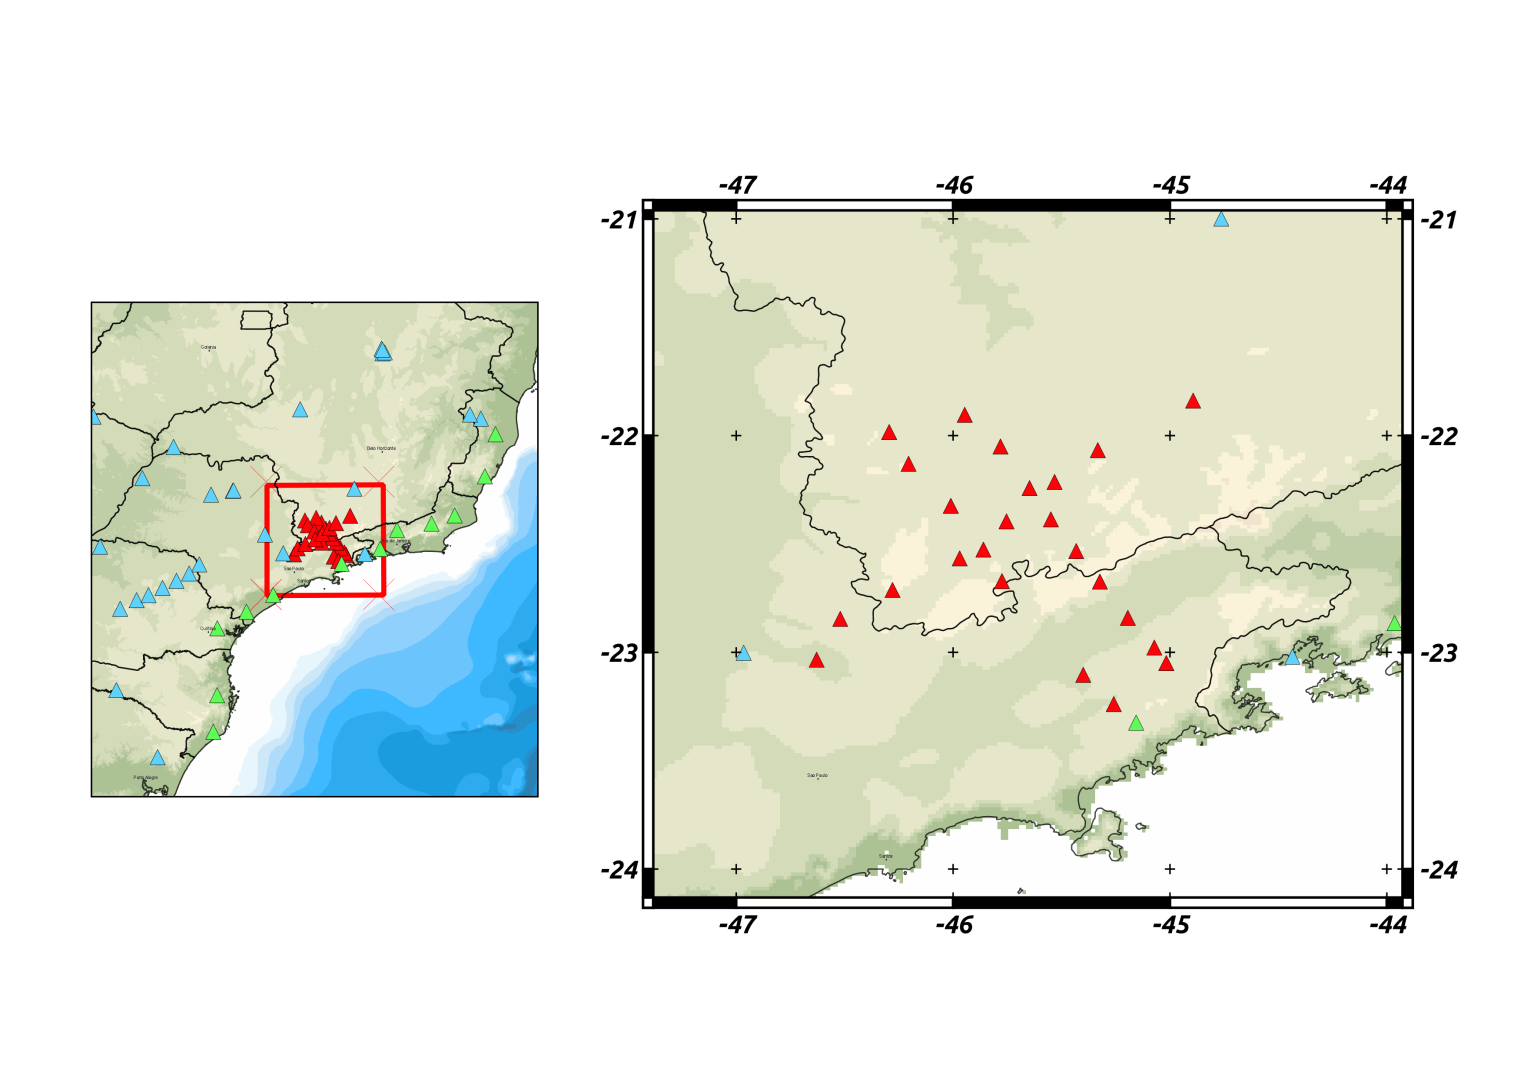
\includegraphics[scale=0.4]{mapa_das_estacoes_simosgraficas_instaladas.png}
\caption{Mapa das estações sismográficas instaladas (triângulos vermelhos). Os outros triângulos são estações da Rede Sismográfica Brasileira.}
\label{map_loc}
\end{figure}

O período de operação das estações foi distinto para os perfis. Os dois perfis perpendiculares à costa foram instalados no meio do ano de 2012 e o perfil paralelo no final de 2012. As estações ficaram em fucionamento até o final do ano de 2013 registrando o movimento do terreno de maneira contínua. 

O produto do deslocamento das partículas do meio registrado pelo sismógrafo, através de sensores verticais e horizontais em três componentes, pode ser visto na Figura \ref{simograma}. Esse registro da variação da amplitude em uma série temporal é chamado de sismograma. 

\begin{figure}[!ht]
\centering
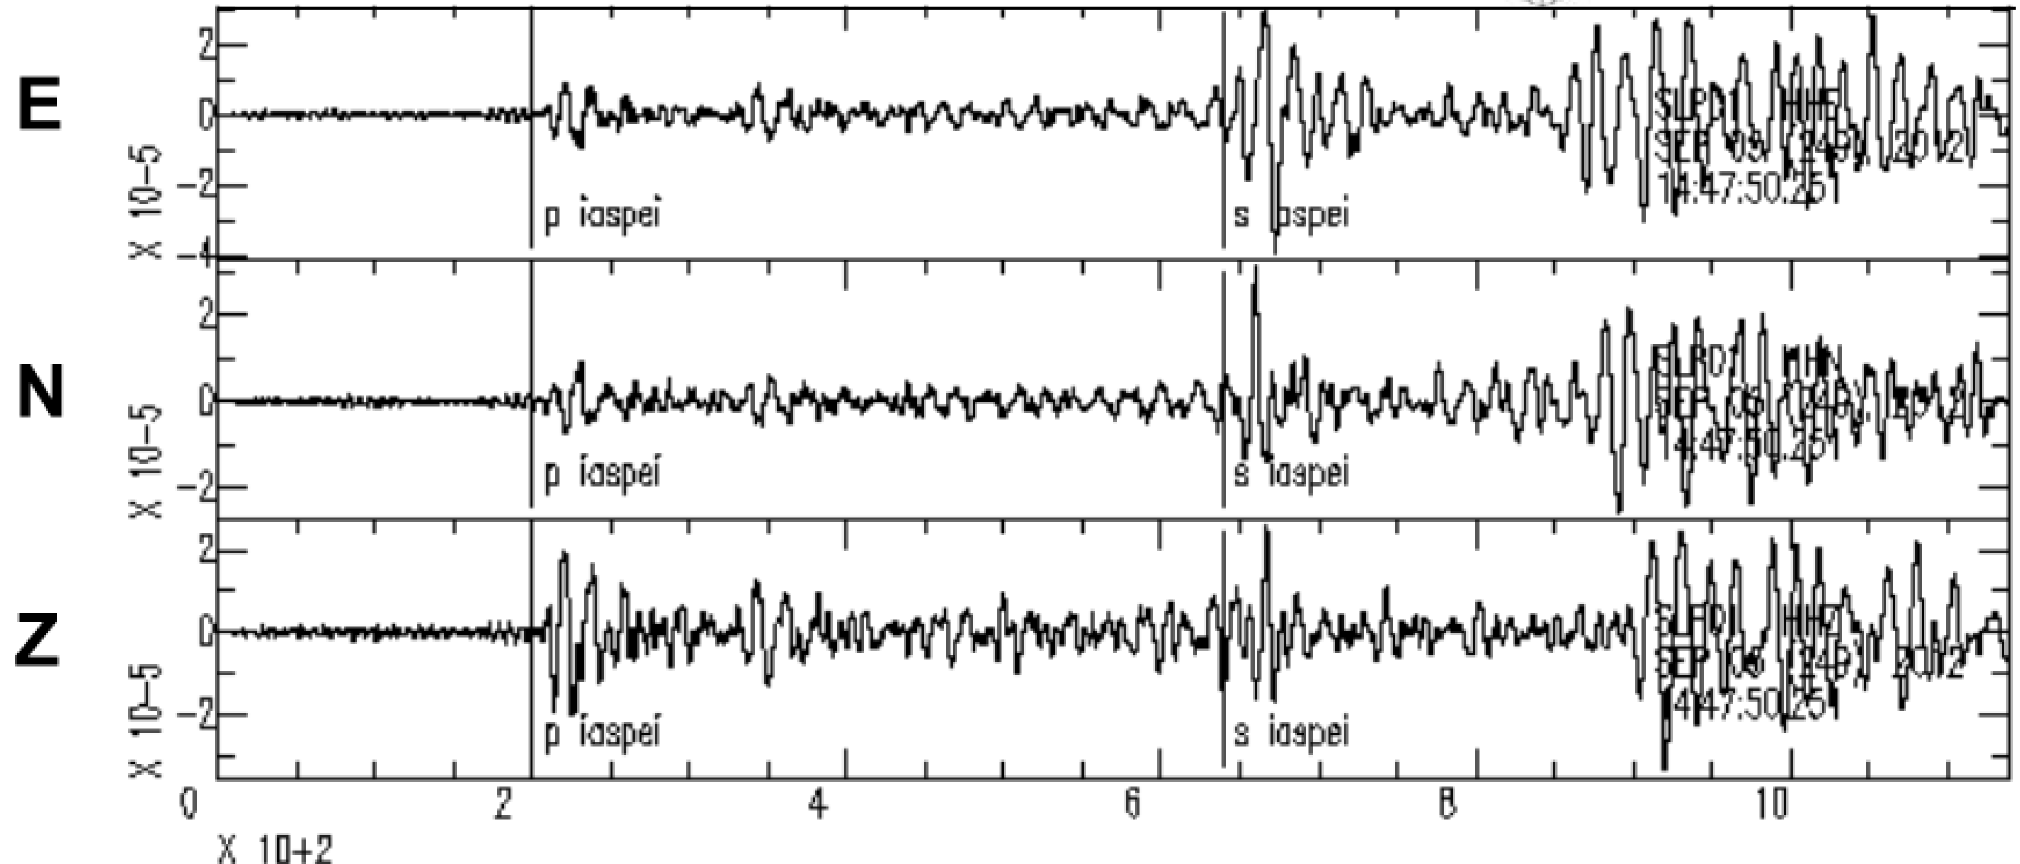
\includegraphics[scale=0.6]{sismograma.png}
\caption{Sismograma mostrandos as três componentes do deslocamento do terreno.}
\label{simograma}
\end{figure}

O sismograma é gerado pela perturbação do meio pelas ondas  mecânicas que se propagam no interior da Terra. Essas ondas  tem velocidades variando em função dos parâmetros elásticos do meio e da densidade. E estes variam pela mineralogia e condições de pressão e temperatura do meio atravessado. As ondas mecânicas são divididas em ondas de corpo e de superfície. As ondas de corpo estão categorizadas em dois tipos: as ondas P, longitudinal, e as ondas S, transversais. A onda P é mais rapida e que consegue se propagar em todos os meios, tem velocidade entre 4 e 7 km$/$s na crosta terrestre e em torno de 8 km$/$s no manto superior. As ondas S tem velocidade menor do que a onda P, em torno de 3 a 4 km$/$s na crosta.

Para produzir esta análise sobre a estrutura da região de estudo utilizou-se de um conjunto de dados com eventos sísmicos registrados. O número de eventos utilizados no processamento varia devido ao nível de sinal-ruído da forma da onda, pois há uma necessidade de visualização clara da chegada da onda P, como pode ser constatado na Figura \ref{simograma} .

\subsection*{Pré-processamento}

Para assegurar a confiabilidade do processamento é necessário um tratamento preliminar dos sinais brutos. Utilizou-se eventos catalogados na rede IRIS para uma identificação automática nestes sinais. Alguns pré-requisitos foram utilizados para a escolha dos eventos, como:

\begin{enumerate}
\item Distância Epicentral;
\item Magnitude;
\end{enumerate}

Sismos próximos, com distância menor que 20 graus da estação estudada, geram ondas com incidência oblíqua e esse tipo de dado deve ser utilizado com cuidado. Em sismos com distâncias maiores que 95 graus as ondas P não chegam na estação devido a inversão de velocidade no limite manto-núcleo, diminuição da velocidade da onda P entre o manto e o núcleo, e não é observada a onda P direta. Por isso a distância epicentral é tida como ideal entre 20 e 95 graus, como é observado na Figura \ref{mapa_eventos}. Devido grande parte dos sismos serem oriundos da Cordilheira dos Andes,como é visto na Figura \ref{teste_tempo}, também utilizou-se dados comn distância menor que 20 graus. A magnitude do sismo é importante para a propagação da onda, eventos com pequena magnitude não tem energia suficiente para gerar energia suficiente para gerar um sinal claro no sismograma.

\begin{figure}[!ht]
\centering
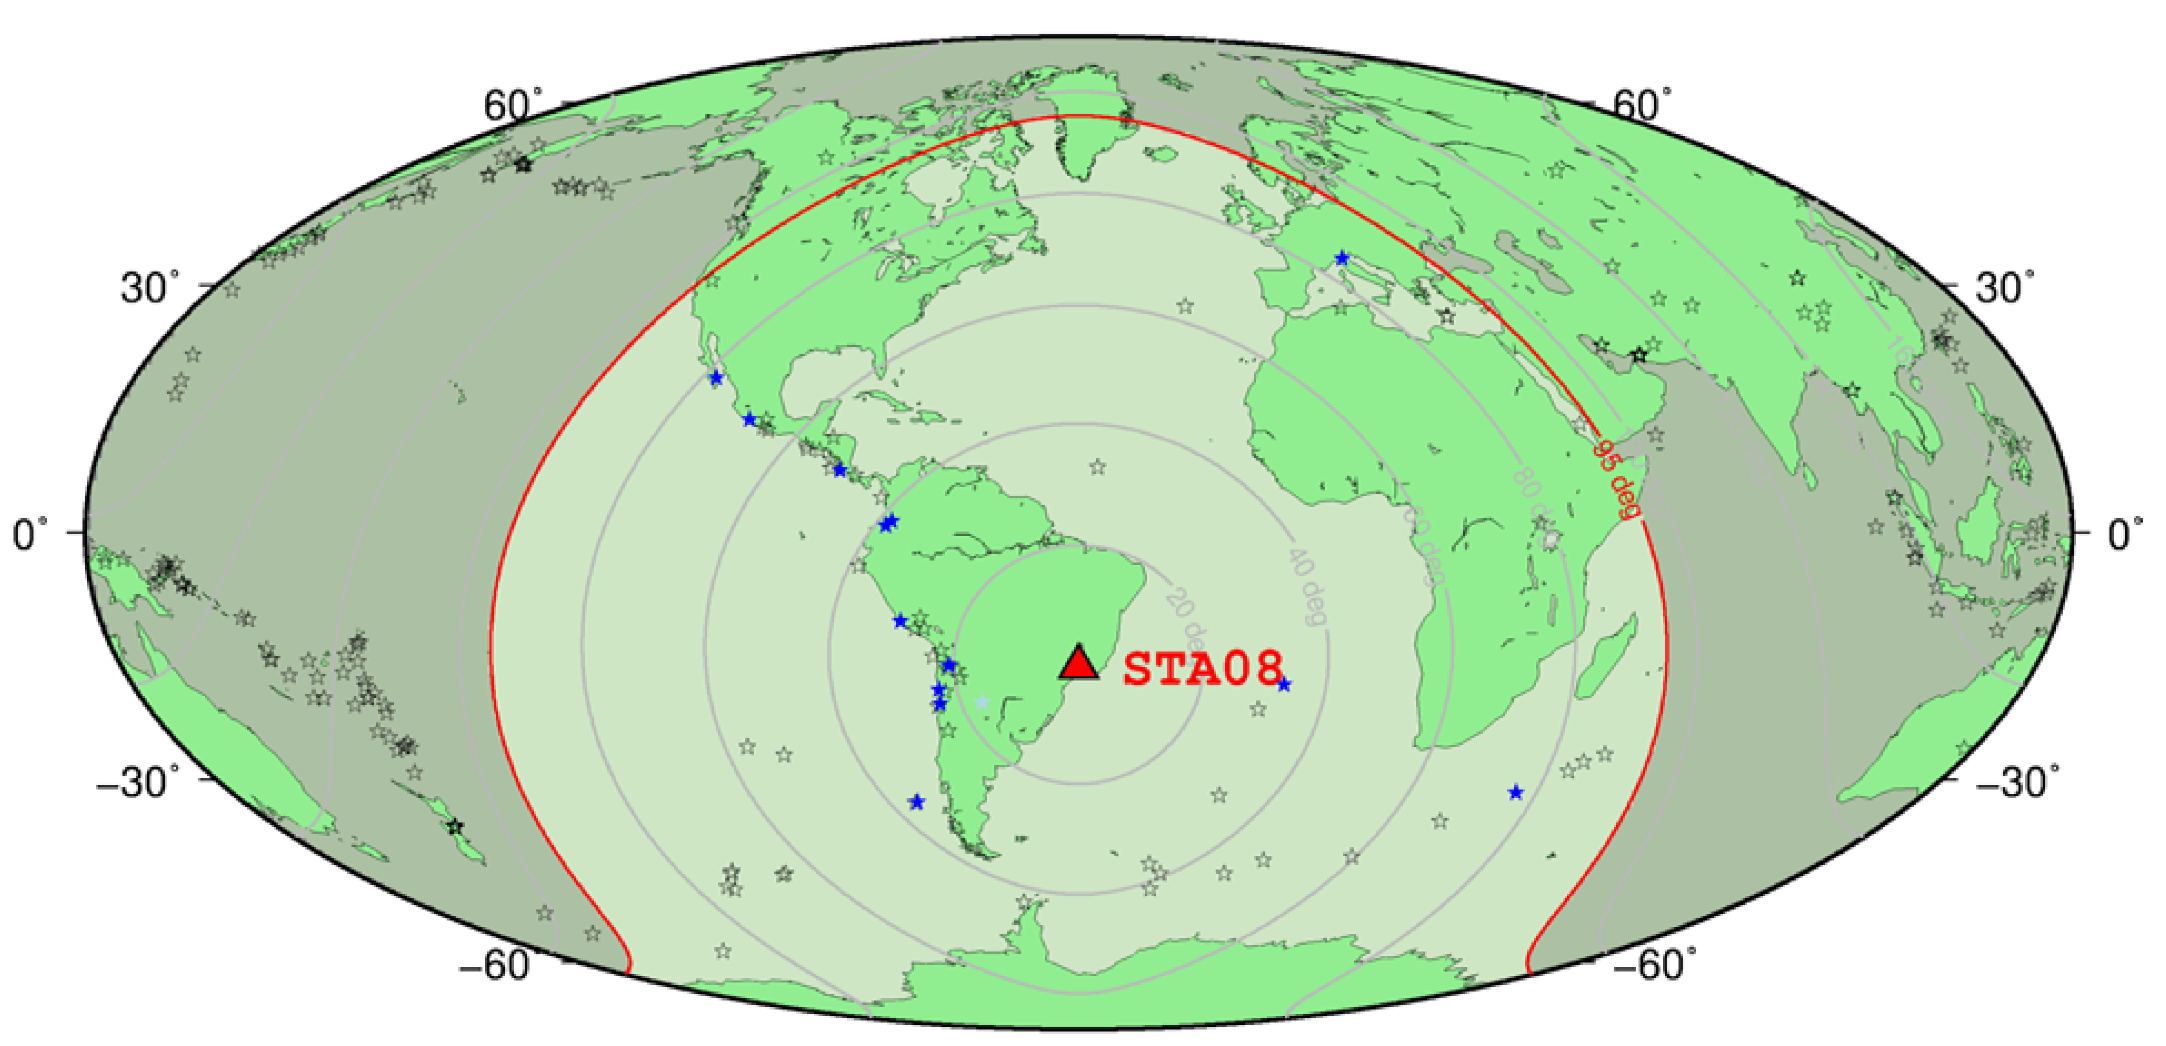
\includegraphics[scale=0.6]{mapa_de_eventos.png}
\caption{Mapa dos eventos (estrelas) registrados na estação STA08. O limite de 95 graus está indicada em vermelho. Estrelas azuls mostram os eventos com dados de qualidade que são usadas no calculo das Funçoes do Receptor}
\label{mapa_eventos}
\end{figure}


Subsequentemente um janelamento do registro em 5 segundos antes e 10 segundos depois da chegada da onda P, esta é calculada pelo modelo de velocidade da Terra  IASPEI91 \citep{kennet_iaspei_1991}. Após a discriminação e o janelamento do sinal, examina-se visualmente cada registro para certificar que todos os eventos selecionados tem um nível de sinal-ruído bom, como na Figura \ref{simograma} . 

Logo após removeu-se a média e tendência linear dos dados. Aplicou-se um filtro passa-alta com freqüência de corte de 0.1 Hz para eventos com distância entre 20 e 95 graus e de 2 Hz para eventos próximos (<20). Os dados originais com amostragens a cada 0,01 segundos (100 Hz) são interpolados para gerar dados com amostragens cada 0,025 segundas (40 Hz), porque a informação de alta freqüência não é relevante nesse tipo de análise.

\subsection*{Processamento}

A caracterização prévia das informações contidas no sinal é imprescindível para o processamento. A avaliação da performance e da qualidade dos dados da estações sismográficas foram feitas no software livre PQLX.  A metodologia do PQLX é baseada no trabalho de \cite{McNamara_Buland_2004}. Esse procedimento é bastante usado para se obter a informação espectral sísmica.

No programa PQLX a série temporal é segmentada em intervalos de uma hora, com 50\% de superposição do sinal. Cada janela de hora está separada em 13 intervalos com 75\% de superposição para calcular a “Power Spectral Density”. As médias obtidas para cada um dos 13 intervalos são usadas para estimar a “Probability Density Functions”, calculados a partir das médias pelo número total de segmentos de hora em hora. 

Essa metodologia de \cite{McNamara_Buland_2004} difere dos métodos habitualmente utilizados, porque não é necessário a visualização de todo conjunto de dados para uma estima qualitativa do sinal, observado na Figura \ref{PQLX}.

\begin{figure}[!ht]
\centering
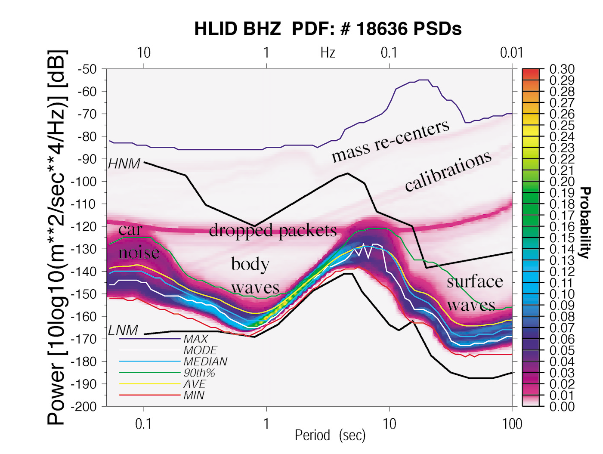
\includegraphics[scale=0.8]{mcnamura_buland.png}
\caption{Análise qualitativa do sinal atraves das \textit{Power Density Functions}. \cite{McNamara_Buland_2004} }
\label{PQLX}
\end{figure}

A garantia da fiabilidade do tempo de chegada da onda P é fundamental para o processamento gerar resultados consistentes. Portanto testes com o tempo de chegada da onda P forão feitos. \cite{gibbons_identification_2006} mostra que fazendo a correlação de dois eventos distantes em uma estação sismográfica consegue-se caracterizar esse tempo de chegada, como é visto na Figura \ref{teste_tempo}. \cite{gibbons_identification_2006} assume que  se não há alterações mensuráveis na velocidade da estrutura entre a fonte e os receptores, ondas sísmicas de dois eventos co-localizados terá a mesma duração de tempo para chegar a um determinado sensor. A função de correlação cruzada para um dado sinal a uma dada estação mede que a semelhança entre a porção posterior do sismograma é a do modelo de forma de onda. O tempo de separação entre o início do modelo e o valor máximo da função de correlação cruzada deve ser igual ao tempo que separa os dois tempos de origem dos eventos para todas as estações. Qualquer discrepância nos tempos de separação medido em duas estações diferentes, o que não é atribuível a diferença entre fontes ou uma SNR baixa, deve ser o resultado de uma anomalia em sincronismo um, ou ambos, dos instrumentos.

Nesste trabalho utilizamos uma metodologia semelhante a de \cite{gibbons_identification_2006}. Utilizou-se um sismo distante de um par de estações sismográficas próximas. Com os sinais registrados fez-se a correlação cruzada dos dados. Como a fonte está distante das estações a correlação dos sinais deve ser próxima de zero. Este teste do tempo de chegada da onda P é para garantir a confiabilidade dos dados das estações temporárias. Portanto em cada par de estações correlacionadas sempre tinha uma estação permanente, estação com dados confiáveis.

\begin{figure}[!ht]
\centering
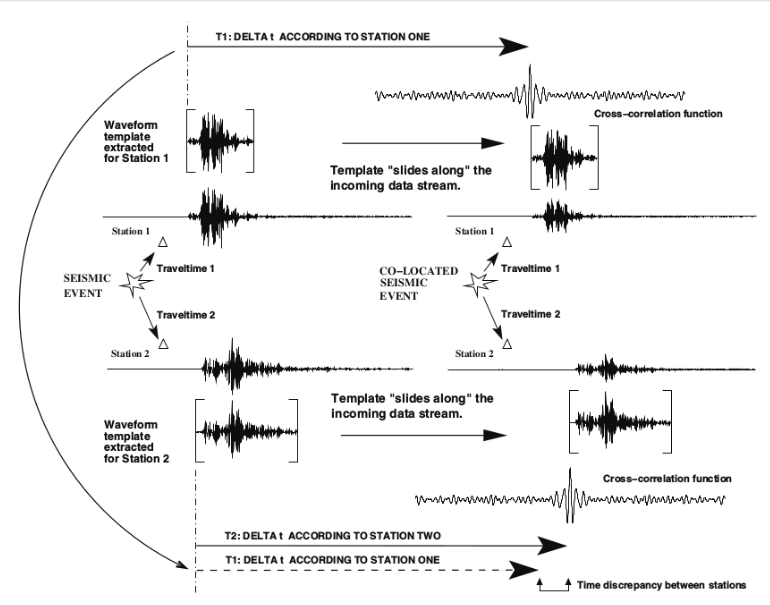
\includegraphics[scale=0.6]{correlacao_tempo_de_chegada.png}
\caption{Uma ilustração esquemática de como dois eventos sucessivos de fontes sísmicas quase idênticas que podem ser explorados para revelar anomalias dos tempo de chegada da onda P numa dada estação. \citep{gibbons_identification_2006}}
\label{teste_tempo}
\end{figure}

No ínicio desse trabalho somente os dados de eventos incluídos no catálogo do IRIS (\textit{Incorporated Research Institutions for Seismology}) com magnitude maior que 5,5 entre maio de 2011 e maio de 2012 foram utilizados. Porém agora utiliza-se dados coletados na rede Sismográfica, mostrada na \ref{map_loc}, até o fim do segundo semestre de 2013. A Figura \ref{mapa_eventos} mostra eventos sísmicos registrados na estação STA08 mostrando a delimitação dos eventos pela distância epicentral, além de mostrar sismos com magnitude maior que 5.5 mb.

O sismômetro registra pequenas variações horizontais e verticais de amplitude das partículas do terreno na escala microscópica ao longo das direções Vertical (Z), Norte-Sul (N) e Leste-Oeste (E), chamado sistema ZNE, como observado na Figura \ref{simograma}. No entanto, o sinal bruto nas direções ZNE não está alinhado aos eixos de propagação das ondas geradas pelo sismo, logo a resposta em cada componente mostra uma sobreposição de vários tipos de ondas. Com a finalidade de isolar a contribuição de cada onda registrada nos dados, o sistema de coordenadas dos registros são rotacionadas, através do SAC (\textit{Seismic Analysis Code}), para se alinharem com os eixos de propagação das ondas através da seguinte matriz de rotação:
\
\[
\left[ \begin{array}{c} R \\ T \\ Z \end{array} \right] = \begin{bmatrix} \cos \theta & \sin \theta & 0 \\ - \sin \theta & \cos \theta & 0 \\ 0 & 0 & 1 \end{bmatrix} \left[ \begin{array}{c} E \\ N \\ Z \end{array} \right]
\]
\

O resultado dessa rotação discrimina claramente a contribuição de cada componente  no sismograma. A componente N (norte-sul) transforma-se na componente T (transversal) e guarda os registro da componente horizontal da onda S, chamada de onda SH. A resposta da onda SV é resgistrada na componente radial do sismograma, chamada R, como pode ser visualizada na Figura \ref{sismo_radial}.   

\begin{figure}[!ht]
\centering
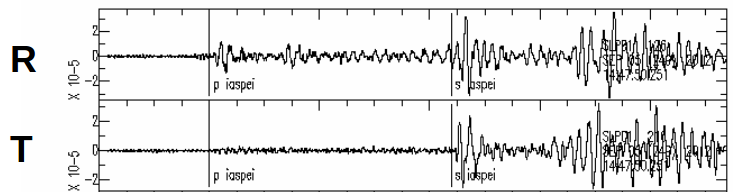
\includegraphics[scale=0.6]{Componente_Radial_Transversal.png}
\caption{Sismograma mostrando as componentes Radial e Transversal.}
\label{sismo_radial}
\end{figure}

Para o cálculo a espessura crustal na região utilizou-se o método da Função do Receptor, que foi desenvolvido por \cite{Langston_1977}. O programa SAC (\textit{Seismic Analysis Code}) foi usado para fazer o processamento e o cálculo das Funções Receptores. Tal método faz uso do sinal de tele-sismos, geradores de ondas planas de incidência quase-vertical embaixo de uma dada estação. A onda P incide na discontinuidade de Mohorovicic e se decompõe em uma onda P transmitida e uma onda S convertida. A diferença do tempo de chegada das duas ondas, onda S tem velocidade inferior a onda P, e de outras reflexões permite inferir a profundidade da discontinuidade de Mohorovicic, também chamada de Moho, como mostrado na Figura \ref{funcoes_sinteticas} .

\begin{figure}[!ht]
\centering
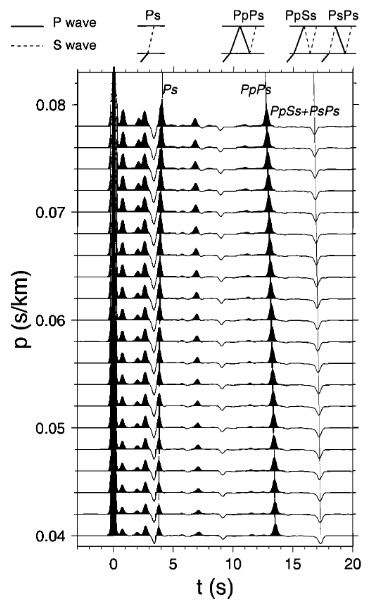
\includegraphics[scale=0.8]{funcoes_sinteticas.png}
\caption{Funções do Receptor em função do parâmetro do raio para o Modelo de Velocidade Padrão do Sul da Califórnia, em \cite{Zhu_Kanamori_2000}. A fase Ps convertida em Moho e suas múltiplas  PpPs, PpSs, e PsPs e seus traços são ilustrados no topo da imagem. Outras reflexões não-rotuladas são as conversões P-S em 5.5 km e 16 km, discontinuidades intracrustais no modelo.}
\label{funcoes_sinteticas}
\end{figure}

Para uma estimativa precisa das Funções do Receptor é essencial que o tempo de chegada da onda P seja determinado com exatidão. Então os dados foram examinados visualmente para registrar o tempo de chegada da onda P direta. 

As Funções do Receptor são calculadas com uma deconvolução componente radial (R) pela componente vertical (Z), como é mostrado por \cite{clayton_source_1976}, \cite{Langston_1977}, \cite{ammon_isolation_1991}, \cite{cassidy_numerical_1992}, \cite{Zhu_Kanamori_2000}. Essa operação remove efetivamente a resposta instrumental, a assinatura da fonte e a propagação da fonte até Moho. E o sinal resultante é a assinatura da propagação próxima à estação. Então a Função do Receptor é sensível na delimitação da estruturação superficial da crosta embaixo da estação.

A deconvolução da componente radial (R) pela componente vertical (Z) pode ser feita no domínio do te



Um método robusto de análise das Funções do Receptor é o método de \cite{Zhu_Kanamori_2000}. Usando as velocidades medianas na crosta, as diferenças de tempo entre a P direta e a P convertida em S podem ser calculadas, bem como os tempos das múltiplas. Usando uma dada velocidade v p , os tempos de chegada podem ser calculados usando a profundidade de Moho (H), a razão v p /v s e o parâmetro do raio, este é dependente da localização do evento e da profundidade. Ao invés de tentar ajustar toda a função, o método faz uma pesquisa, grid search, da espessura crustal e da razão v p /v s para calcular o tempo de chegada teórico das ondas P convertidas em S e das múltiplas para cada registro. A melhor combinação da espessura crustal e da razão v p /v s é aquela que maximiza o valor das amplitudes reais das funções receptor. Para obter uma imagem das discontinuidades, como por exemplo Moho, as Funções do Receptor empilhadas são mapeadas em relação a posição da estação no perfil. 

Os dados são separados em 4 grupos, segundo o azimute entre o sismo e a estação. A maioria do eventos ocorrem na região noroeste e sudoeste, nota-se a escassez de eventos na região do Oceano Atlântico. O objetivo dessa separação é avaliar se existem variações laterais de estrutura.


\section*{Dispersão de Ondas de Superfície}
\subsection*{Dados Geofísicos}
\subsection*{Fundamentos Teóricos}